\documentclass[19pt,landscaoe]{article}
\usepackage[landscape]{geometry}
\geometry{a5paper,scale=0.8}
%\geometry{left=1.5cm,right=1.5cm,top=1.5cm,bottom=0.5cm}
\usepackage{color}
% \usepackage{ulem} % for strikethrough
\usepackage{amsfonts}
\usepackage{bm}
\usepackage{graphicx} 
\usepackage{amsfonts,amsmath,latexsym,amssymb,mathrsfs,amsthm,mathtools}
% \usepackage[british]{babel}
%\usepackage[T1]{fontenc}
%\usepackage{mathptmx}
% \usepackage{times}
\usepackage{datetime2}
\usepackage{filemod}
% \usepackage{fontspec}    %change font 
% \setmainfont{Times New Roman}%fontspec下这个命令设置全局默认字体
\newtheorem{thm}{Theorem}%[section]
\newtheorem{prop}[thm]{Proposition}
\newtheorem{defi}[thm]{Definition}
\newtheorem{lma}[thm]{Lemma}
\newtheorem{cor}[thm]{Corollary}
\newtheorem{exam}[thm]{Example}
\newtheorem{countexam}[thm]{Counterexample}
\newtheorem{rem}[thm]{Remark}
\newtheorem{con}[thm]{Conjecture}
%\bracketfactory{floor}{\lfloor}{\rfloor}
\usepackage{enumerate}
\usepackage{color}
%\usetheme{Copenhagen}
\usepackage[english]{babel}
\usepackage[utf8x]{inputenc}
\newcommand{\law}{\mathscr{L}}
\newcommand{\HH}{\mathscr{H}}
\newcommand{\D}{\mathbb{D}}
\newcommand{\IP}{\mathbb{P}} 
\newcommand{\bone}{{\bf 1}}
\DeclareMathOperator{\E}{\mathbb{E}}
\DeclareMathOperator*{\esssup}{ess\,sup}
\newcommand{\IE}{\E}
\newcommand{\mean}{\E}
\newcommand{\R}{\mathbb{R}}
\newcommand{\N}{\mathbb{N}}
\newcommand{\non}{\nonumber}
\newcommand{\Z}{\mathbb{Z}}
\newcommand{\C}{\mathbb{C}}
%\newcommand{\C}{{\mathds{C}}}
\newcommand{\ci}{{\cal I}}
\newcommand{\cf}{{\cal F}}
\newcommand{\LL}{\textbf{L}}
\DeclareMathOperator{\Var}{\mathrm{Var}}
\DeclareMathOperator{\var}{\mathrm{Var}}
\DeclareMathOperator{\cov}{\mathrm{Cov}}
\DeclareMathOperator{\corr}{\mathrm{Corr}}
\DeclareMathOperator{\bs}{\mathrm{Bias}}
\DeclareMathOperator{\bigo}{\mathrm{O}}
\newcommand{\K}{\textbf{Ker}}
\newcommand{\Id}{\textbf{Id}}
\newcommand{\Pn}{{\rm Pn}}
\newcommand{\dtv}{{d_{\rm TV}}}
\newcommand{\dk}{{d_{\rm K}}}
\newcommand{\dw}{{d_{\rm W}}}
\def\tg{{\tilde g}}
\def\a{{\alpha}}
\def\cn{{\mathcal{N}}}
\def\equald{\stackrel{\mbox{\scriptsize{{\rm d}}}}{=}}
\def\ER{Erd\H{o}s-R\'enyi}
\usepackage{color} 
\definecolor{lightblue}{rgb}{0,0.2,0.5}
\usepackage[colorlinks=true, urlcolor=lightblue,linkcolor=lightblue, citecolor=lightblue]{hyperref}

%%%%%%%%%%%%%%%%%%%%%%%%%%%%%%%%%%

%%% Define bracket commands
\def\given{\mskip 0.5mu plus 0.25mu\vert\mskip 0.5mu plus 0.15mu}
\newcounter{@bracketlevel}
\def\@bracketfactory#1#2#3#4#5#6{
\expandafter\def\csname#1\endcsname##1{%
\addtocounter{@bracketlevel}{1}%
\global\expandafter\let\csname @middummy\alph{@bracketlevel}\endcsname\given%
\global\def\given{\mskip#5\csname#4\endcsname\vert\mskip#6}\csname#4l\endcsname#2##1\csname#4r\endcsname#3%
\global\expandafter\let\expandafter\given\csname @middummy\alph{@bracketlevel}\endcsname
\addtocounter{@bracketlevel}{-1}}%
}
\def\bracketfactory#1#2#3{%
\@bracketfactory{#1}{#2}{#3}{relax}{0.5mu plus 0.25mu}{0.5mu plus 0.15mu}
\@bracketfactory{b#1}{#2}{#3}{big}{1mu plus 0.25mu minus 0.25mu}{0.6mu plus 0.15mu minus 0.15mu}
\@bracketfactory{bb#1}{#2}{#3}{Big}{2.4mu plus 0.8mu minus 0.8mu}{1.8mu plus 0.6mu minus 0.6mu}
\@bracketfactory{bbb#1}{#2}{#3}{bigg}{3.2mu plus 1mu minus 1mu}{2.4mu plus 0.75mu minus 0.75mu}
\@bracketfactory{bbbb#1}{#2}{#3}{Bigg}{4mu plus 1mu minus 1mu}{3mu plus 0.75mu minus 0.75mu}
}


% \title{Nonparametric Regression}
% \author{Qingwei Liu}
% \institute{National University of Singapore}
% \date{\today}

\begin{document}
% \maketitle
%

% \begin{titlepage}
% \begin{center}
%     \vfill
% \textbf{\huge ST5207 Nonparametric Regression\\
% Semester 1, AY2024/25}\\[4cm]
% \begin{minipage}{0.4\textwidth}
% \begin{center} \large
% Lecturer:~Qingwei Liu\\
% % Email:liu\_qw@nus.edu.sg\\
% \vskip 6pt
% Department of Statistics and Data Science\\
% \vskip 6pt
% National University of Singapore
% \end{center}
% \end{minipage}%\\[1cm]
% \vfill
% % \includegraphics[width=0.1\textwidth]{./logo}\\[0.5cm]
% \vfill
% \end{center}

% \end{titlepage}
%

\newpage
\centering{\LARGE\textbf{Lecture~2:~Histogram Method} for nonparametric density estimation\footnote{Last modified in \filemodprintdate{Lecture2}.}}
\vskip25pt
\begin{minipage}{.9\textwidth}
    \Large
\begin{itemize}
\item The Empirical  Distribution Function Estimator
\item The naive Estimator 
\item The Histogram Estimator  
\item Asymptotics of the Histogram Estimator 
\item Bin number selection

\end{itemize}
\end{minipage}
\newpage
{\Large\centerline{\textbf{Problem}}}
\vskip25pt
\begin{minipage}{.9\textwidth}
    \Large
Let $X$ be a continuous random variable with cumulative distribution function (c.d.f.) $F$ and p.d.f. $f$.
(Both c.d.f. and p.d.f. characterize the distribution.)
In practice, the distribution of $X$ is in general unknown. All you have are $n$ observations $X_1,\dots,X_n$ of $X$, in other words, i.i.d. samples with size $n$. 
\vskip 10pt
{\bf Problem:}~~~How do you estimate $f(\cdot)$ using those samples? 
\vskip 5pt
Note, we don't assume that $f(\cdot)$ has some known functional form except for some unknown parameter(s) that need to be estimated. (That is exactly the parametric approach.)
\vskip 5pt
We will focus on nonparametric ways of estimating $f(\cdot)$ instead. 
% In one hand, we know from second-year probability theory,
% \begin{equation}
%     f(x)=\frac{\mathrm{d}F(x)}{\mathrm{d}x}=\lim_{h\to0}\frac{F(x+h)-F(x-h)}{2h}
% \end{equation}
\end{minipage}

\newpage
{\LARGE\centerline{\textbf{Empirical distribution function}}}
\vskip25pt
\begin{minipage}{.9\textwidth}
    \Large The simplest function to estimate nonparametrically is the c.d.f. $F$ of random variable $X$. 
From elementary probability theory, the {\it empirical distribution function} (EDF), defined as, for any $x\in\R$, 
\begin{equation}
    F_n(x):=\frac1n\sum_{i=1}^n\bone_{\{X_i\le x\}},
\end{equation}
is a straightforward estimator for $F(x)$. 
\vskip 5pt
For any fixed $x\in\R$, $\bone_{\{X_i\le x\}}$ is a Bernoulli RV with mean $F(x)$. As a consequence, $F_n(x)$ is a RV with mean 
\begin{equation*}
    \E[F_n(x)]=\E\left(\bone_{\{X_1\le x\}}\right)=\IP(X_1\le x)=F(x),
\end{equation*}
and variance 
\begin{equation*}
    \Var(F_n(x))=\frac1{n^2}\cdot n\Var(\bone_{\{X_i\le x\}})=\frac1nF(x)\left(1-F(x)\right).
\end{equation*}
\end{minipage}

\newpage
{\LARGE\centerline{\textbf{A native estimator}}}
\vskip25pt
\begin{minipage}{.9\textwidth}
    \Large 
    Therefore, $F_n(x)$ is a {\it consistent unbiased} estimator of $F(x)$. 

    \vskip 5pt
    In particular, EDF allocates equal weight $n^{-1}$ on each datum point.
    \vskip 5pt
    On the other hand, inspired by EDF, it is easy to write 
    \begin{eqnarray*}
        f(x)&=&\lim_{h\to0}\frac{F(x+h)-F(x-h)}{2h}\\
        &=&\lim_{h\to0}\frac{\E\left[\bone_{\{x-h<X_i\le x+h\}}\right]}{2h}\\
        &=&\lim_{h\to0}\E\left[\frac{\sum_{i=1}^n\bone_{\{x-h<X_i\le x+h\}}}{2nh}\right].
    \end{eqnarray*}
    Hence, we obtain a {\it native estimator} for the density function $f(\cdot)$, 
\begin{equation}\label{def-nat}
    \hat{f}_n(x):=\frac1{2nh}\sum_{i=1}^n\bone_{\{x-h<X_i\le x+h\}},
\end{equation}
    for some $h>0$ small. 
\end{minipage}

\newpage
{\LARGE\centerline{\textbf{Histogram Estimator}}}
\vskip25pt
\begin{minipage}{.9\textwidth}
    \Large
The histogram is the oldest and the most commonly used nonparametric density estimator. The construction of histogram is almost the same as the naive estimator.  
\begin{itemize}
   \item Choose an origin $x_0$, and {\it binwidth} $h>0$;
   \item Denote the {\it bins} of the histogram as 
   $$B_j:=[x_0+jh,x_0+(j+1)h),~~~j\in\Z.$$
\end{itemize}
The histogram is given by 
\begin{equation}\label{def-hist}
    \widehat{f}_h(x):=\frac1{nh}\sum_{i=1}^n\sum_{j}\bone_{\{X_i\in B_j\}}\bone_{\{x\in B_j\}}.
\end{equation}
\end{minipage}
% \newpage
% {\LARGE{\textbf{Parametric Modeling}}}
% \vskip25pt
% {\Large\bf{Examples}}
   
% \begin{figure}[h]
% 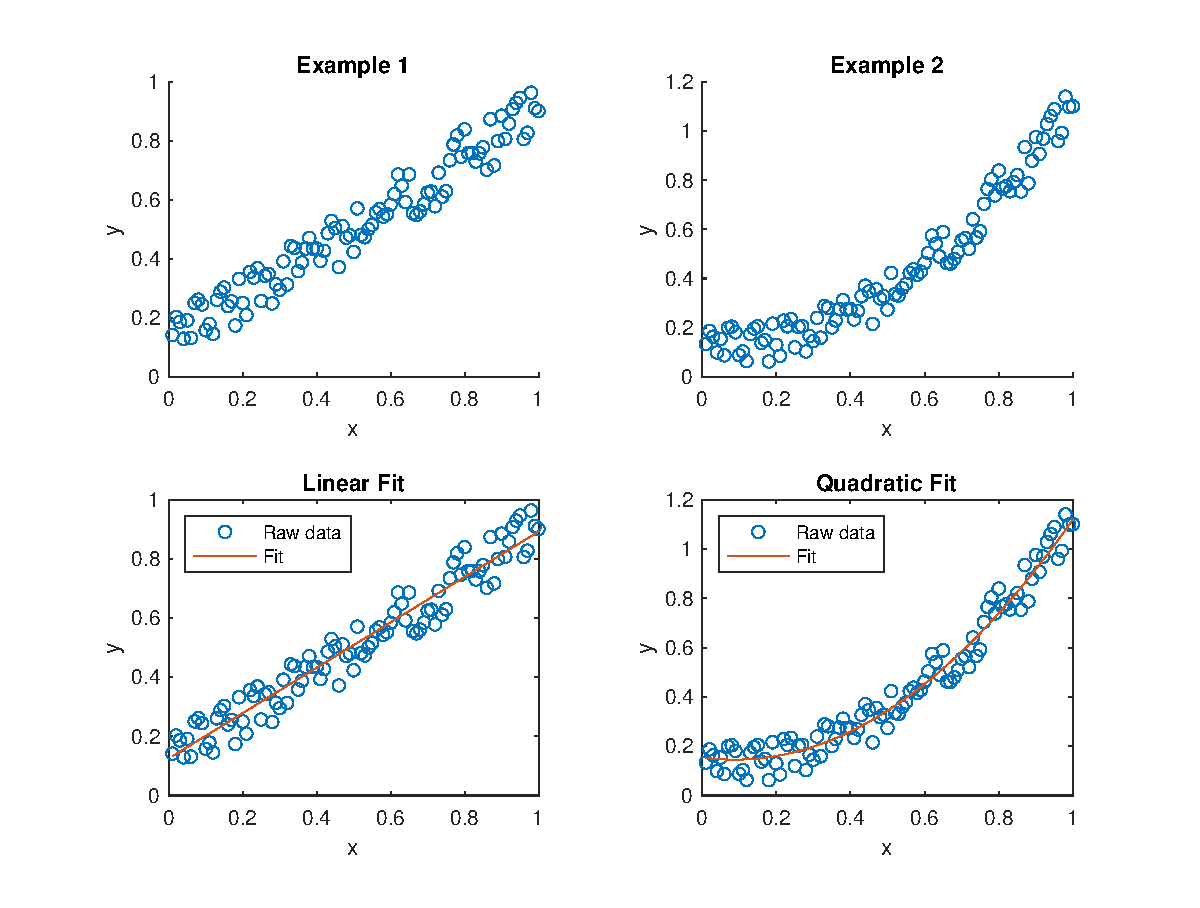
\includegraphics[width=0.8\textwidth,height=0.5\textwidth]{figure1.eps}
%     \label{figure1} 
% \end{figure}

\newpage
{\LARGE{\textbf{Comparsion of Naive and Histogram}}}
\vskip25pt
\begin{minipage}{.9\textwidth}
    \Large 
    We may assume  $x_0=0,$ and $x\in B_j=[jh,(j+1)h]$, without loss of generality (w.l.o.g.), and rewrite \eqref{def-hist} as  
    \begin{equation}\label{refine-hist}
        \widehat{f}_h(x):=\frac1{nh}\sum_{i=1}^n\bone_{\{X_i\in B_j\}}.
    \end{equation}
    Comparing \eqref{def-nat} with \eqref{refine-hist}, we can see 
    % \Large
\begin{itemize}
\item The naive estimator is defined in a pointwise manner. For each $x$ fixed, take a neighborhood of $x$ with fixed radius $h$.
\item Bins appeared in \eqref{def-hist} is independent of $x$, and purely determined by the selection of origin $x_0$ and binwidth $h$.
\end{itemize}
\end{minipage}

% \newpage
% {\LARGE{\textbf{Parametric Modeling}}}
% \vskip25pt
% {\Large\bf{Scatter plot of raw data}}

% \begin{figure}[h]
% \centering
% 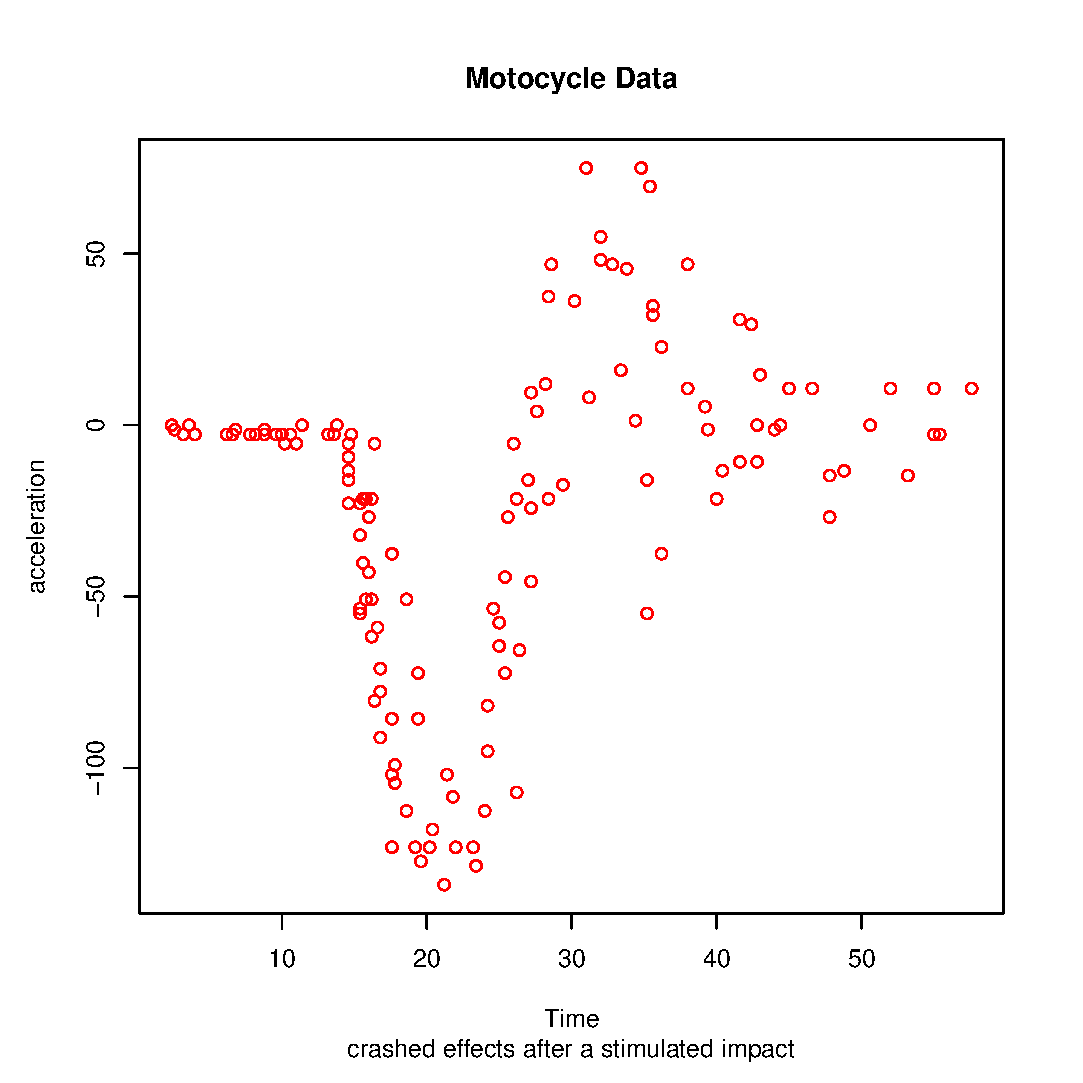
\includegraphics[width=0.75\textwidth,height=0.52\textwidth]{MotocycleData.eps}
%     \label{figure2} 
% \end{figure}

% \newpage
% {\LARGE{\textbf{Parametric Modeling}}}
% \vskip25pt
% {\Large\bf{Polynomial Fit}}

% \begin{figure}[h]
% \centering
%       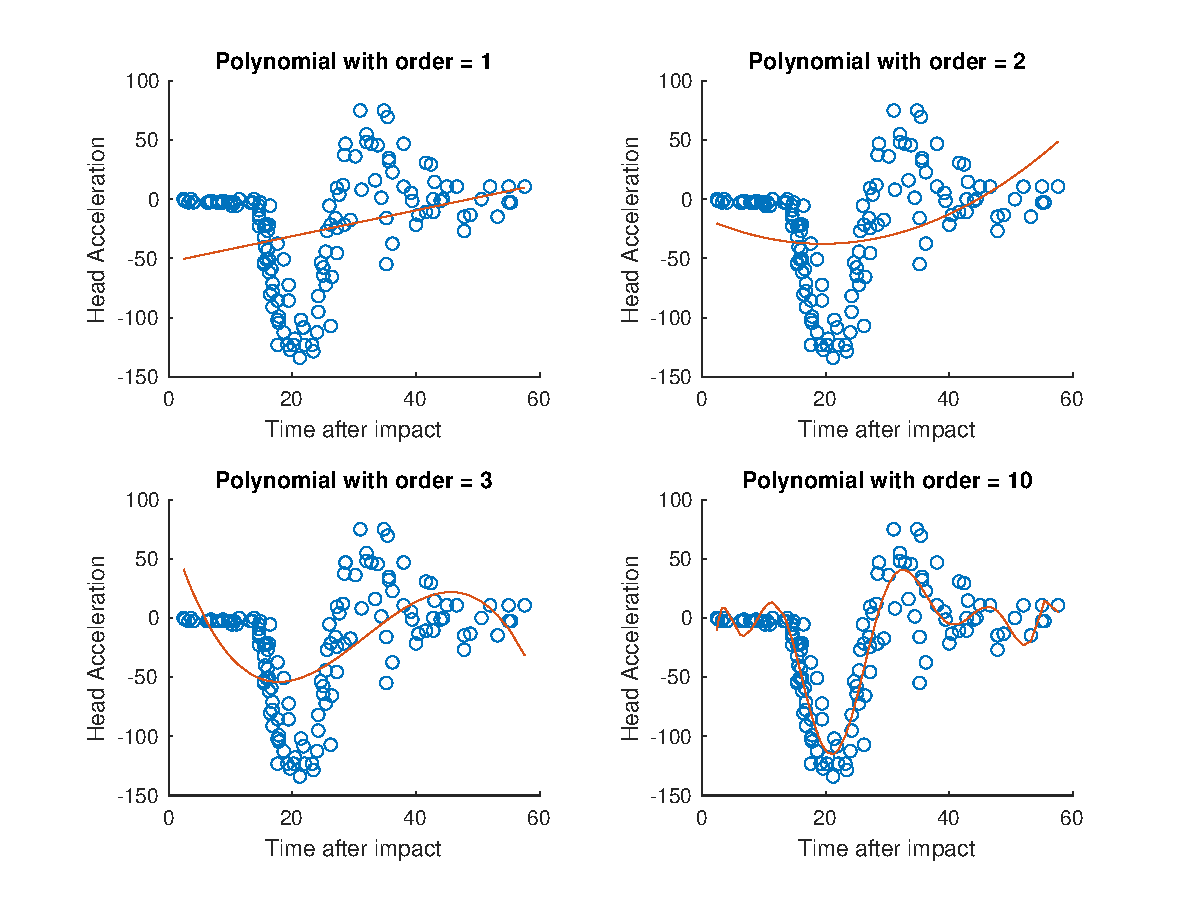
\includegraphics[width=0.75\textwidth,height=0.52\textwidth]{polyfitting.eps}
%     \label{figure3} 
% \end{figure}

\newpage
{\LARGE\centerline{\textbf{Statistical Properties}}}
\vskip25pt
\begin{minipage}{.9\textwidth}
    \Large
    \begin{itemize}
        \item Bias: 
        \begin{eqnarray}
            \bs\left\{\widehat{f}_h(x)\right\}&=&\E\left[\widehat{f}_h(x)\right]-f(x)\nonumber\\
            &=&h^{-1}\IP\left(X_1\in B_j\right)-f(x)\nonumber\\
            &=&\frac1h\int_{B_j}f(u)\mathrm{d}u-f(x)\nonumber\\
            &=&f(u^*)-f(x),\label{bs-mvt}
        \end{eqnarray}
        where the last equity is due to the Mean Value Theorem for some $u^*\in B_j$. 
    \end{itemize}
Intuitively, we may think the bias will vanish as the binwidth $h\to0$. Nope. We need certain {\bf stronger} condition on the density function $f(\cdot)$ to ensure this. So far, we only assume the existence of $f(\cdot)$.
\end{minipage}

\newpage
{\LARGE\centerline{\textbf{Statistical Properties (cont.)}}}
\vskip25pt
\begin{minipage}{.9\textwidth}
    \Large
    \begin{itemize}
        \item Variance:
        \begin{eqnarray}
            \var\left(\widehat{f}_h(x)\right)&=&\frac1{(nh)^2}\var\left(\sum_{i=1}^n\bone_{\{X_i\in B_j\}}\right)\nonumber\\
            &=&(nh^2)^{-1}\var\left(\bone_{\{X_1\in B_j\}}\right)\nonumber\\
            &=&(nh^2)^{-1}p_x(1-p_x)\\
            &=&(nh)^{-1}f(u^*)(1-p_x)\label{var-bound1}
        \end{eqnarray}
        where $p_x:=\int_{B_j}f(u)\mathrm{d}u$.
    \end{itemize}
From the last equality, it is not difficult to see that for $n$ fixed 
$$\var\left(\widehat{f}_h(x)\right)\to\infty,~~~~\mathrm{as}~~~h\to0.$$ 
\end{minipage}


\newpage
{\LARGE\centerline{\textbf{Continuity condition and MSE}}}
\vskip25pt
\begin{minipage}{.9\textwidth}
    \Large
        For a function $g:\R\to\R$, suppose that for any $x,y\in\R$, it holds 
        \begin{equation}
            |g(x)-g(y)|\le K|x-y|^\alpha,
        \end{equation}
        for some $\alpha>0$. 
        For $\alpha=1$, such functions are called {\it Lipschitz functions}. For $0<\alpha<1$, they are said to satisfy a {\it H\"older condition} of order $\alpha$, c.f.\cite[Page~56]{Dudley02}. 
\vskip 5pt
        For a function $g$ defined on a finite interval $[a,b]$ with $a<b$, 
        $$\mathrm{Lipschitz~continous}\Rightarrow \mathrm{H\ddot{o}lder~continuous}\Rightarrow \mathrm{uniformly~continuous}.$$
Mean Square Error (MSE) of $\widehat{f}_h(x)$, defined by 
\begin{eqnarray}
    {\rm MSE}\left\{\widehat{f}_h(x)\right\}:=\E\left[\left|\widehat{f}_h(x)-f(x)\right|^2\right],
\end{eqnarray}
is a widely used performance measure of an estimator. 
\end{minipage}

\newpage
{\LARGE\centerline{\textbf{Main Theorem}}}
\vskip25pt
\begin{minipage}{.9\textwidth}
    \large
\begin{thm}
    Suppose the density function $f$ is Lipschitz continuous on the interval $B_j$. When $n^{-1}\ll h\ll1$, the histogram $\widehat{f}_h(x)$ converges to $f(x)$, in the mean square sense,  i.e. 
    \begin{equation}
        {\rm MSE}\left\{\widehat{f}_h(x)\right\}\to0,
    \end{equation}
    as $n\to\infty$.
\end{thm}
\begin{proof}
    Since $f$ is Lipschitz continuous on $B_j$, from \eqref{bs-mvt}, we have
    \begin{equation}\label{bs-bound}
        \left|\bs\left\{\widehat{f}_h(x)\right\}\right|=\left|f(u^*)-f(x)\right|\le K|u^*-x|\le Kh.
    \end{equation}
    Furthermore, from \eqref{var-bound1}, we have 
    \begin{equation}\label{var-bound2}
        \var\left(\widehat{f}_h(x)\right)\le C(nh)^{-1}
    \end{equation} for some constant $C$, 
    as $f$ is bounded on $B_j$, implied by the Lipschitz continuity. Combining \eqref{bs-bound} with \eqref{var-bound2}, we have
    \begin{equation} 
        {\rm MSE}\left\{\widehat{f}_h(x)\right\} =\left(\bs\left\{\widehat{f}_h(x)\right\}\right)^2+\var\left(\widehat{f}_h(x)\right)\le K^2h^2+C(nh)^{-1}\to0.
    \end{equation}
\end{proof}
{\small An easy trick: $E(X-a)^2=\E(X-\E(X)+\E(X)-a)^2=\Var(X)+(\E(X)-a)^2$.}
\end{minipage}

\newpage
{\LARGE\centerline{\textbf{Nonparametric Methods}}}
\vskip25pt
\begin{minipage}{.9\textwidth}
    \Large Can be classified as 
\begin{enumerate}
\item classical nonparametric methods, which are based on signs and ranks developed in 1940s--1970s;
\item modern nonparametric methods, includes:
\begin{itemize}
    \item Smoothing methods, such as kernel, spline, orthogonal series for curve estimation, including density, regression curves. (Note: A curve can be regared as a parameter of infinite dimensions.)
    \item The Jackknife, Bootstrap and other resampling methods. 
\end{itemize}
\end{enumerate}
The course is mostly around the smoothing method and the curves we considered includes the density 
    % $$f(x)=\frac{\mathrm{d}F(x)}{\mathrm{d}x},$$
    and the conditional mean function.
\end{minipage}

\newpage
{\LARGE\centerline{\textbf{A toy example}}}
\vskip25pt
\begin{minipage}{.9\textwidth}
    \Large 
Suppose $\big\{(X_i,Y_i)\big\}_{i=1}^n$ is an i.i.d. sequence, with conditional mean function
$$m(x)=\E(Y_i|X_i=x)$$ 
and conditional variance $$\sigma^2(x)=\Var(Y_i|X_i=x).$$
Consider the regression 
\begin{equation}\label{L1-eq1}
    Y_i=m(X_i)+\varepsilon_i.
\end{equation}
Apparently, we have 
$$\E(\varepsilon_i|X_i)=0,$$ and
$$\E(\varepsilon_i^2|X_i)=\Var(Y_i|X_i)=\sigma^2(X_i).$$
Besides, $X_i$ and $\varepsilon_i$ are uncorrelated, i.e. orthogonal in $L^2$, but \textcolor{red}{not independent}.  (See the couterexample at the end of this slide.) 
\end{minipage}

\newpage
{\LARGE{\textbf{Example: (continue)}}}
\vskip25pt
\begin{minipage}{.9\textwidth}
    \Large 
The model in \eqref{L1-eq1} is a nonparametric regression model with the following features:
\begin{itemize}
    \item Unspecified function form for the conditional mean function $m$;
    \item Unspecified form for the distribution of $(X_i,Y_i)$ and $\varepsilon_i$;
    \item Varying variance component $\sigma^2(X_i)$.
\end{itemize}
All of those features generalizes the parametric (linear and nonlinear) regression model to more general and practical setting. 
\end{minipage}

\newpage
{\LARGE{\textbf{Nonparatric model}}}
\vskip15pt
\begin{minipage}{.9\textwidth}
    \Large 
Let $g(x,y)$ be the joint p.d.f. of $(X,Y)$. (suppose it exists of course!) The marginal p.d.f. of $X$ is 
$$f_X(x):=\int_{\R}g(x,y)\mathrm{d}y,$$
and the conditional p.d.f. of $Y$ is 
$$f_{Y|X}(y|x):=\frac{g(x,y)}{f_X(x)}.$$
The conditional mean function is closely related with the marginal density of $X$, as 
\begin{eqnarray*}
    m(x):=\E(Y|X=x)=\int_{\R}yf_{Y|X}(y|x)\mathrm{d}y=\frac1{f_X(x)}\int_{\R}yg(x,y)\mathrm{d}y.
\end{eqnarray*}

This course will start with nonparametric density estimation, and then the nonparametric estimation of the conditional mean function. 
\end{minipage}


% \newpage
% {\LARGE{\textbf{Nonparametric Modeling}}}
% \vskip25pt
% {\Large\bf{Regression Spline Fit}}

% \begin{figure}[h]
% \centering
%       \includegraphics[width=0.75\textwidth,height=0.52\textwidth]{splinefit.pdf}
%     \label{figure4} 
% \end{figure}

\newpage
{\LARGE\centerline{\textbf{Counterexample}}}
\vskip25pt
\begin{minipage}{.9\textwidth}
    \Large 
    Let $p,p_1,p_2\in(0,1)$ be some constants, and $p_1\ne p_2$. Consider $X,Y$ with following distributions: 
$X\sim Bernoulli(p)$, i.e. 
$$\IP(X=1)=1-\IP(X=0)=p,$$
and $Y\sim Bernoulli(p_1)$ given $X=1$, while $Y\sim Bernoulli(p_2)$ given $X=0$. Therefore, 
$$\E(Y|X)=p_1\cdot X+p_2\cdot(1-X),$$
$$\varepsilon:=Y-\E(Y|X)=Y-[p_1\cdot X+p_2\cdot(1-X)].$$
The conditional distribution of $\varepsilon$ is
$$\IP(\varepsilon=1-p_1|X=1)=1-\IP(\varepsilon=-p_1|X=1)=p_1,$$
and  
$$\IP(\varepsilon=1-p_2|X=0)=1-\IP(\varepsilon=-p_2|X=0)=p_2.$$
\textcolor{red}{$X$ and $\varepsilon$ are not independent, but uncorrelated.}
\end{minipage}

\newpage
{\LARGE\centerline{\textbf{Counterexample(continue)}}}
\vskip25pt
\begin{minipage}{.9\textwidth}
    \Large 
    By the law of total probability, 
    \begin{equation*}
        \varepsilon=\begin{cases}
            1-p_1,~~~&\mathrm{w.p.}~~p_1p,\\
            -p_1,~~~&\mathrm{w.p.}~~(1-p_1)p,\\
            1-p_2,~~~&\mathrm{w.p.}~~p_2(1-p),\\
            -p_2,~~~&\mathrm{w.p.}~~(1-p_2)(1-p),
        \end{cases}
    \end{equation*}
 and  $\E(\varepsilon)=0$. Hence, we have 
   \begin{eqnarray*}
    \cov(X,\varepsilon)&=&\E(X\varepsilon)\\
    &=&p\E(\varepsilon|X=1)\\
    &=&p[(1-p_1)p_1+(-p_1)(1-p_1)]\\
    &=&0.
   \end{eqnarray*}
\end{minipage}

\newpage
{\LARGE\centerline{\textbf{Landau's symbol}}}
\vskip25pt
\begin{minipage}{.9\textwidth}
   \Large
   We also recall the following standard notation for the asymptotic behavior of the relative order of magnitude of two functions $f(n)$ and $g(n )>0$ as $n$ tends to infinity.
   We write
   \begin{itemize}
      \item
        $f(n)=O(g(n))$,
        or $f(n ) \lesssim g(n )$, if $\limsup_{n \to\infty} f(n ) / g(n ) <\infty$;
      \item
        $f(n)=\Omega(g(n ))$, or 
        $f(n ) \gtrsim g(n )$, if $\liminf_{n \to\infty} f(n) / g(n)>0$;
    % \item       $f(\lambda )=\Theta(g(\lambda ))$ if $f(\lambda )=O(g(\lambda ))$ and $f(\lambda )=\Omega(g(\lambda ))$, 
      \item $f(n)\asymp g(n)$ if $f(n)=O(g(n))$ and $f(n)=\Omega(g(n))$; % if $f(\lambda )=\Theta(g(\lambda ))$;
  % \item $f(\lambda )\sim g(\lambda )$ if $\lim_{\lambda \to \infty} f(\lambda )/g(\lambda ) = 1$, 
     \item $f(n)=o(g(n))$, if $f(n)/g(n)\to 0$;
  %    \item $f(x)\ll g(x)$, or $g(x)\gg f(x)$ if $f(x)\ge0$ and $f(x)=o(g(x))$.
      \item $f(n)\ll g(n)$, or $g(n)\gg f(n)$, if $f(n)\ge0$ and $f(n)/g(n)\to 0$.
  \end{itemize}
  Find more details in this Wikipedia page of \href{https://en.wikipedia.org/wiki/Big_O_notation#History_(Bachmann–Landau,_Hardy,_and_Vinogradov_notations)}{Big O notation}.
\end{minipage}







\newpage
\bibliographystyle{apalike}
\bibliography{../ref}
% \begin{thebibliography}{}

%     \bibitem[Hall, 2013]{Hall13}
%     Hall, P. (2013).
%     \newblock {\em The bootstrap and Edgeworth expansion}.
%     \newblock Springer Series in Statistics. Springer New York, NY.
    
%     \bibitem[H{\"a}rdle et~al., 2004]{hardle04}
%     H{\"a}rdle, W., M{\"u}ller, M., Sperlich, S., Werwatz, A., et~al. (2004).
%     \newblock {\em Nonparametric and semiparametric models}, volume~1 of {\em Springer Series in Statistics}.
%     \newblock Springer Berlin, Heidelberg.
    
%     \bibitem[Kloke et~al., 2015]{kloke14}
%     Kloke, J., McKean, J.~W., and McKean, J.~W. (2015).
%     \newblock {\em Nonparametric statistical methods using R}.
%     \newblock Chapman and Hall/CRC, 1st ed edition.
    
%     \bibitem[Schmidt et~al., 1981]{schmidt81}
%     Schmidt, G., Mattern, R., and Sch{\"u}ler, F. (1981).
%     \newblock Biomechanical investigation to determine physical and traumatological differentiation criteria for the maximum load capacity of head and vertebral column with and without protective helmet under the effects of impact.
%     \newblock {\em EEC Research Program on Biomechanics of Impacts, Final report, Phase III, Project G}, 5.
    
%     \bibitem[Silverman, 1985]{Silverman85a}
%     Silverman, B.~W. (1985).
%     \newblock Some aspects of the spline smoothing approach to non-parametric regression curve fitting.
%     \newblock {\em Journal of the Royal Statistical Society: Series B (Methodological)}, 47(1):1--21.
    
%     \bibitem[Takezawa, 2005]{takezawa05}
%     Takezawa, K. (2005).
%     \newblock {\em Introduction to nonparametric regression}.
%     \newblock Wiley Series in Probability and Statistics. John Wiley \& Sons.
    
%     \end{thebibliography}
\end{document}